% \documentclass{ctexbeamer}
\documentclass{beamer}
\usepackage[scheme=plain]{ctex}
\usepackage{amsmath}
% \usepackage{gbt7714}
\usepackage{subfig}
\usepackage{graphicx}
% \usepackage[colorlink=true,xetex]{hyperref}

\usetheme{Madrid}
\bibliographystyle{IEEEtran}

\title{Splay Tree and its Amortized Analysis}
\subtitle{A brief to Splay, the self-balanced binary search tree}
\input{personal_info/authors.tex}

\begin{document}
    \begin{frame}
        \maketitle
    \end{frame}

    \begin{frame}
        \frametitle{Table of Contents}
    
        \tableofcontents
    
    \end{frame}

    \section{Introduction}

    \begin{frame}
        \frametitle{Inventors}
        \framesubtitle{Introduction}
    
        \begin{figure}
            \centering
            \subfloat[Daniel Sleator]{
                \centering
                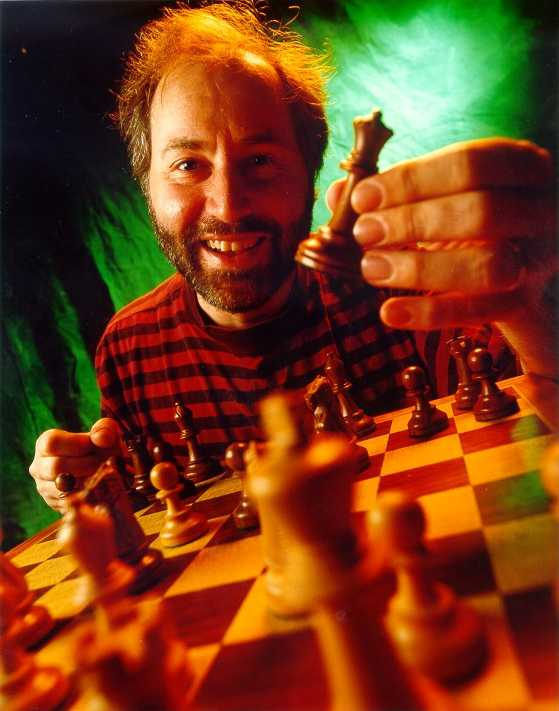
\includegraphics[height=0.6\textheight]{pics/Daniel_Sleator.jpg}
            }
            \qquad
            \subfloat[Robert Tarjan]{
                \centering
                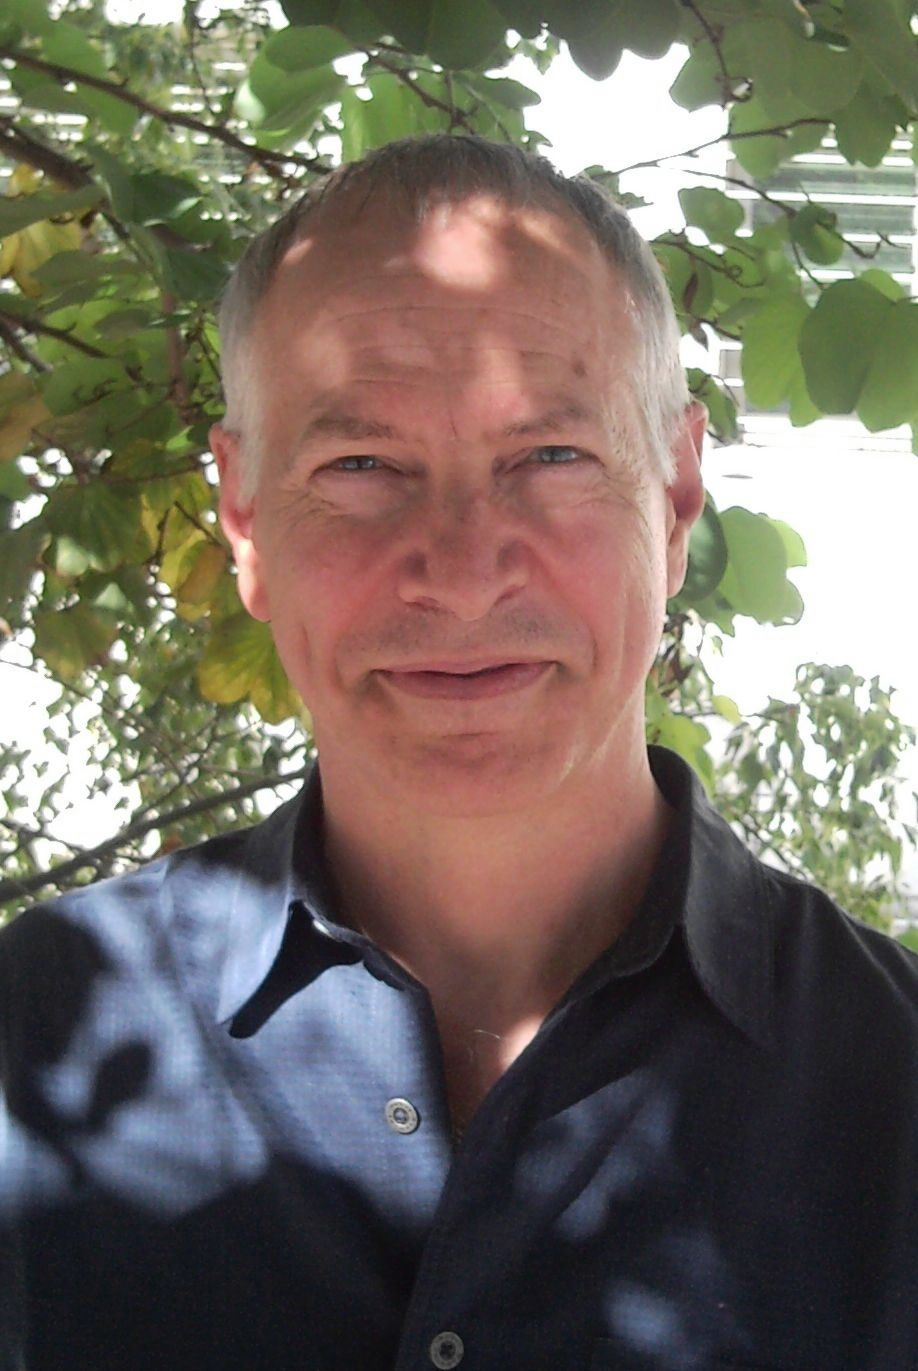
\includegraphics[height=0.6\textheight]{pics/Robert_Tarjan.jpg}
            }
            \caption{The inventors of Splay tree}
        \end{figure}
    
    \end{frame}

    \subsection{Motivation}

    \begin{frame}
        \frametitle{Motivation}
        \framesubtitle{Introduction}
    
        Efficient search trees have various drawbacks\cite{10.1145/3828.3835}:
        \begin{itemize}
            \item Not as efficient as possible if the access pattern is nonuniform;
            \item Need extra space for storage of balance information;
            \item Costs of insertion and deletion of optimum search trees are very high;
            \item Biased search trees are complicated in structure and hard to maintain; \pause
            \item \textbf{Designed to reduce the worst-case time per operation}.
        \end{itemize}
    
    \end{frame}

    \section{Structure and operations}
    \subsection{Structure of Splay tree}
    \subsection{Operations of Splay tree}

    \section{Amortized analysis}

    \section{Applications}

    \bibliography{citations}
\end{document}